%//////////////////////////////////
%/// P R E A M B L E

\documentclass[a4paper, 12pt]{article}

\usepackage[utf8]{inputenc}
\usepackage[singlespacing]{setspace}
\usepackage{amsmath}
\usepackage{mathtools}
\usepackage{caption}
\usepackage{float}
\usepackage{graphicx}
\usepackage{multicol}
\usepackage{gensymb}
\usepackage{breqn}
\usepackage{indentfirst}
\usepackage{tabularx, booktabs}
\newcolumntype{Y}{>{\centering\arraybackslash}X}

\usepackage{pdfpages}

\usepackage{multicol}
\usepackage{supertabular}

\usepackage{svg}

\widowpenalty = 4500
\clubpenalty  = 4500

\setlength{\jot}{10pt} %indents


\newcommand*\dif{\mathop{}\!\mathrm{d}}

%%========================================
%% circuitikz properties
\usepackage[european, straightvoltages]{circuitikz}
%\ctikzvalof{voltage/distance from node = .2}
%\ctikzset{voltage/distance from node  =.5}% in \pgf@circ@Rlen units
%\ctikzset{voltage/distance from line  =.25}% pos. between 0 and 1
%\ctikzset{voltage/bump b/.initial     =1.5}%

\ctikzset{current/distance            = .618}


%%========================================

%%
%% Path settings
%%
\graphicspath{ {./graphics/} }


%//////////////////////////////////
%/// D O C U M E N T
\begin{document}

%%%%%%%%%%%%%%%%%%%%%%%%%%%%%%%%%%%%%
  
\includepdf{./titlepage/titlepage.pdf}
%%%%%%%%%%%%%%%%%%%%%%%%%%%%%%%%%%%%%

\section{Vorbereitungsaufgaben}
\subsection{}

  \begin{center}
    \begin{align*}
      i(t) = \hat{I} \cdot \cos(\omega t + \phi_i)
    \end{align*}
  \end{center}

  \vspace{0.013155617496424828\columnwidth}


    %Resistor
  (3)\\
  \begin{center}
    \begin{circuitikz}[european voltages, european resistors]
      \draw (0,0) to[R, l=$R$, i=$i(t)$, v=$u_R(t)$, color = black] (2,0);
    \end{circuitikz}

    \begin{align*}
      u_R(t)  & = R \cdot i(t)\\
              & = \underbrace{R \cdot \hat{I}}_{ \mathclap{\hat{U}_R }} \cdot \cos(\omega t + \phi_i)\\
      \intertext{Da sich die Phase nicht ändert, gilt außerdem $\phi_i = \phi_u$ und somit:}
      \Aboxed{u_R(t)  & = \hat{U} \cdot \cos(\omega t + \phi_u)}\\
    \end{align*}

  \end{center}

  (4)\\
  \begin{center}
    %inductance
    \begin{circuitikz}[european voltages, european inductors]
      \draw (0,0) to[L, l=$L$, i=$i(t)$, v=$u_L(t)$, color = black] (2,0);
    \end{circuitikz}

    \begin{align*}
      u_L(t)  & = L \cdot \frac{\dif i(t)}{\dif t}\\
              & = L  \cdot \hat{I} \cdot \frac{\dif}{\dif t}\left( \cos(\omega t + \phi_i)\right)\\
              & = -\underbrace{ \omega \cdot L \cdot \hat{I} }_{ \mathclap{\hat{U}_L} } \cdot \sin(\omega t + \phi_i)\\
      \intertext{Um die Spannung ($-\sin{x}$) wieder durch $\cos{x}$ auszudrücken, muss auf den ursprünglichen Phasenwinkel $\pi / 2$ addiert werden:}
      \Aboxed{ u_L(t)  & = \hat{U}_L \cdot \cos(\omega t + \underbrace{\phi_i + \frac{\pi}{2}}_{ \mathclap{\phi_u}})}\\
    \end{align*}

  \end{center}

  (5)\\
  \begin{center}
    %capacitance
    \begin{circuitikz}[european voltages, european resistors]
      \draw (0,0) to[C, l=$C$, i=$i(t)$, v=$u_C(t)$, color = black] (2,0);
    \end{circuitikz}

    \begin{align*}
      u_C(t) & = \frac{\hat{I}}{C} \cdot \int_0^t{i(t) \dif t}\\
             & = \frac{\hat{I}}{C} \cdot \int_0^t{ \cos{(\omega t + \phi_i)} \dif t}\\
             & = \frac{\hat{I}}{C} \cdot \frac{1}{\omega} [\sin{(\omega t + \phi_i)}]_0^t + \underbrace{U_0}_{\mathclap{\text{initialer Ladezustand}}}\\
             & = \underbrace{\frac{\hat{I}}{C \cdot \omega}}_{\mathclap{\hat{U}_C}} [\sin{(\omega t + \phi_i)} - \sin{(\phi_i)}] + U_0\\
       \intertext{Um die Spannung ($\sin{x}$) wieder durch $\cos{x}$ auszudrücken, muss von dem ursprünglichen Phasenwinkel $\pi / 2$ subtrahiert werden:}
     \Aboxed{ u_C(t)  & = \hat{U}_C \cdot \left(\cos(\omega t + \underbrace{\phi_i - \frac{\pi}{2}}_{\mathclap{\phi_u}}) - \cos{(\underbrace{\phi_i - \frac{\pi}{2}}_{\mathclap{\phi_u}})}\right) + U_0}\\
    \end{align*}

  \end{center}

%1.2
\subsection{}
  (3)\\
  \begin{gather*}
    u_R(t)   = R \cdot i(t)\\
    i(t)      = \frac{u(t)}{R}\\
  \end{gather*}

  (4)\\
  \begin{gather*}
        u_L(t) = L \cdot \frac{\dif i(t)}{\dif t}\\
    \dif i(t)  = \frac{1}{L} \cdot u_L(t) \dif t\\
        i(t)   = \frac{1}{L} \cdot \int_0^t{u_L(t) \dif t} + i_0\\
  \end{gather*}
  \indent(5)\\
  \begin{gather*}
    u_C(t)   = \frac{1}{C} \cdot \int_0^t{i(t) \dif t}\\
    i(t)     = C \cdot \frac{\dif u_C(t)}{\dif t}\\
  \end{gather*}

%1.3
\subsection{}
  Zur Anwendung der symbolischen Methode werden folgende Bedingungen vorausgesetzt:
  \begin{itemize}
    \item \emph{Linearität}: Die Kenngrößen der Elemente $R, L, C$ sind von den Kenngrößen der Erregung ($U, I, \omega$) unabhängig
    \item Es liegt eine \emph{harmonische Erregung} ($\sin \text{/} \cos$) vor
    \item Der \emph{stationäre Zustand} ist erreicht, das System ist "eingeschwungen" und es treten keine Schaltvorgänge auf
  \end{itemize}

%1.4
\subsection{}
  Der \emph{Betragsgang} ist die Funktion $\text{f}(\omega)$, die den Verlauf des Verhältnisses der Amplituden (komplexer Betrag) oder Effektivwerte zweier Größen (z.B. Aus -und Eingangssignal) mit der (Kreis-)Frequenz abbildet.
  $$ \text{f}(\omega) = \frac{ \mid \underline{U}_2 \mid }{ \mid \underline{U}_1 \mid } =  \frac{ U_{2_eff} }{ U_{1_eff} }$$\\

  Der \emph{Phasengang} $\phi(\omega)$ ist das von der (Kreis-)Frequenz abhängige Argument des komplexen Verhältnisses des Aus- und Eingangssignals.
  $$\phi(\omega) = \text{arg} \left( \frac{ \underline{U}_2 }{ \underline{U}_1 } \right)$$\\

  %\vspace{0.021276873\paperheight}
  Sind Real- und Imaginärteil dieses komplexen Verhältnisses gleich, so wird das Amplitudenverhältnis $1/\sqrt{2}$ und die Phasenverschiebung $45 \degree$. Die dabei präsente Frequenz wird dann \emph{Grenzfrequenz} genannt.
  $$ \text{Re}\left( \frac{ \underline{U}_2 }{ \underline{U}_1 } \right) = \text{Im}\left( \frac{ \underline{U}_2 }{ \underline{U}_1 } \right)$$

%1.5
%\pagebreak
\subsection{}
  Im Folgenden wurden normierte Darstellungen der Betragsgänge gewählt, um von den Kenngrößen unabhängige Graphen zu erhalten. Zusätzlich sind die Abszissen dieser logarithmisch eingeteilt.

  \begin{center}
  \subsubsection*{Hochpassfilter (HP)}

    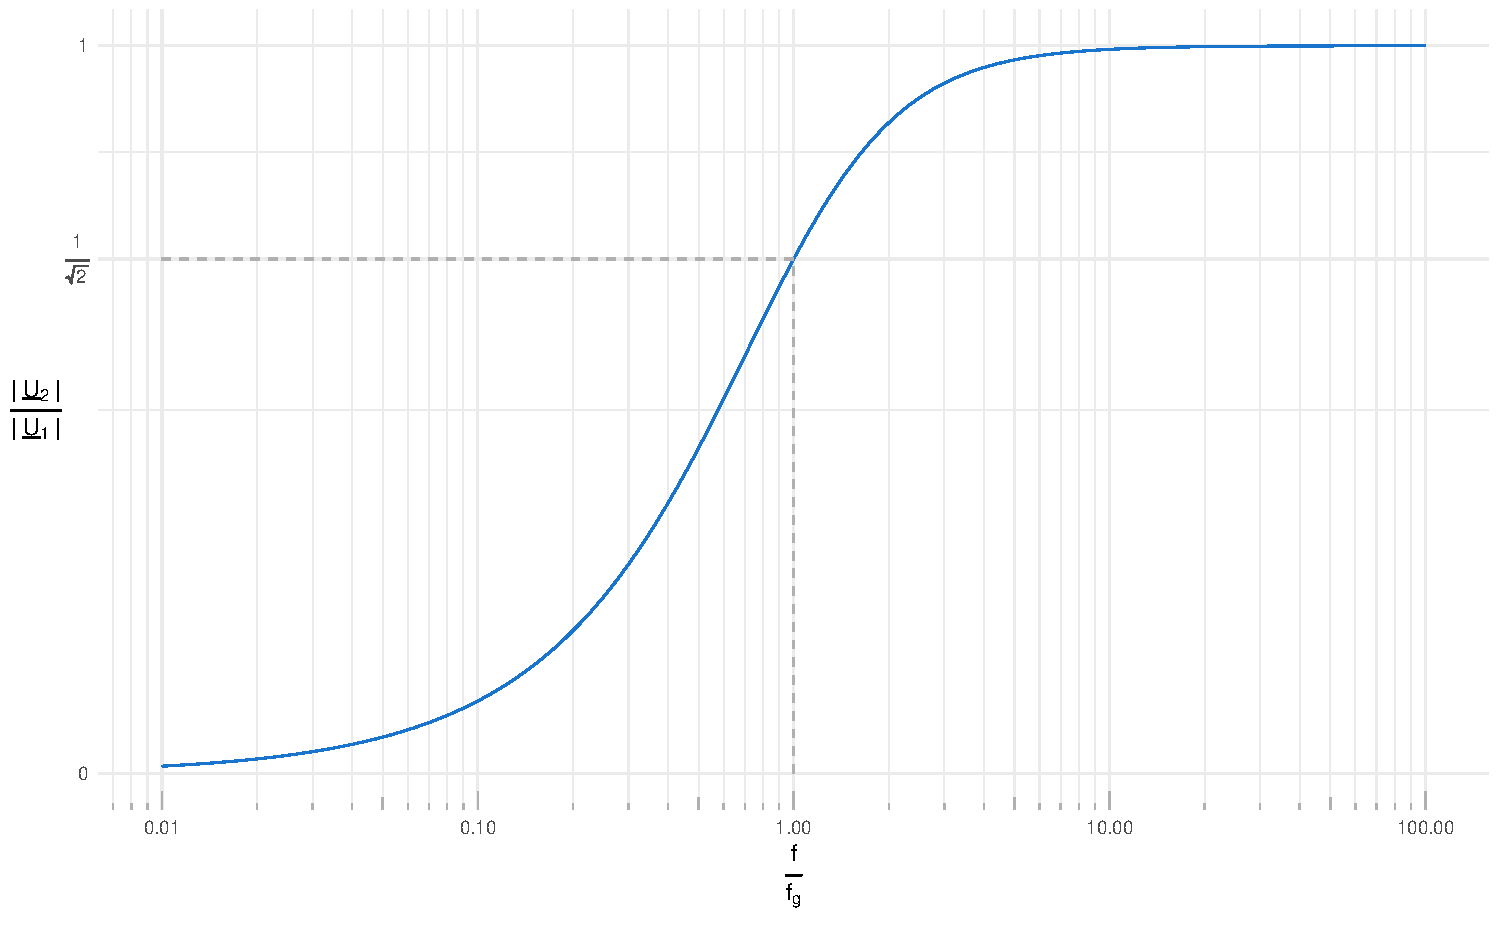
\includegraphics[scale=0.5]{./R/RL_HP/RL_HP_clean_alt.pdf}

  \vspace{0.021276873\paperheight}

  \subsubsection*{Tiefpassfilter (TP)}

    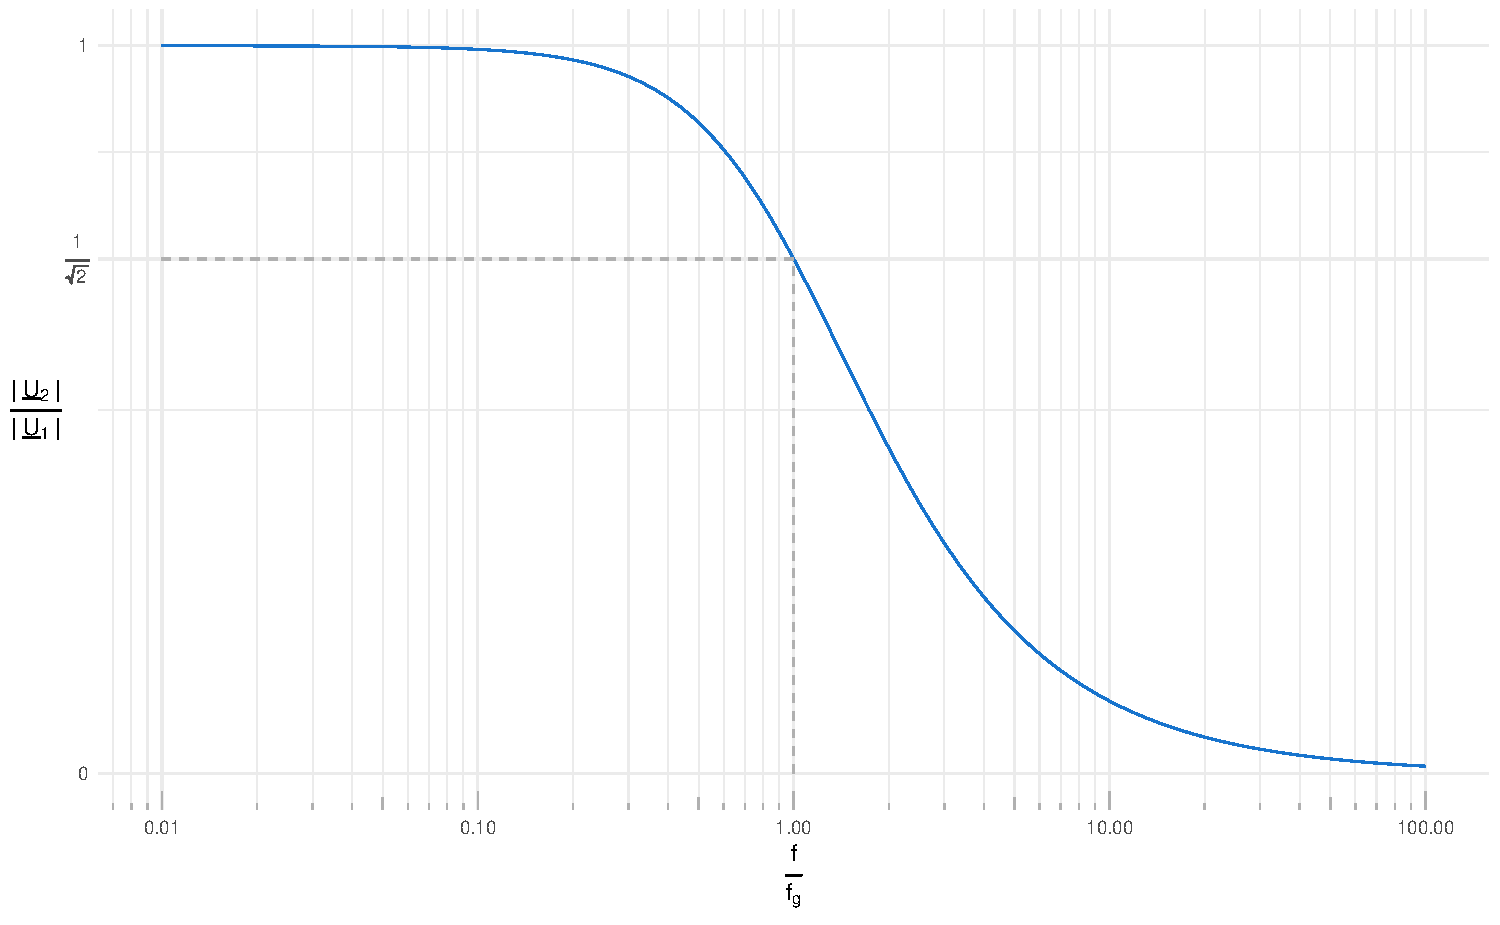
\includegraphics[scale=0.5]{./R/RC_LP/RC_LP_clean.pdf}

  \subsubsection*{Bandpass (BP)}

    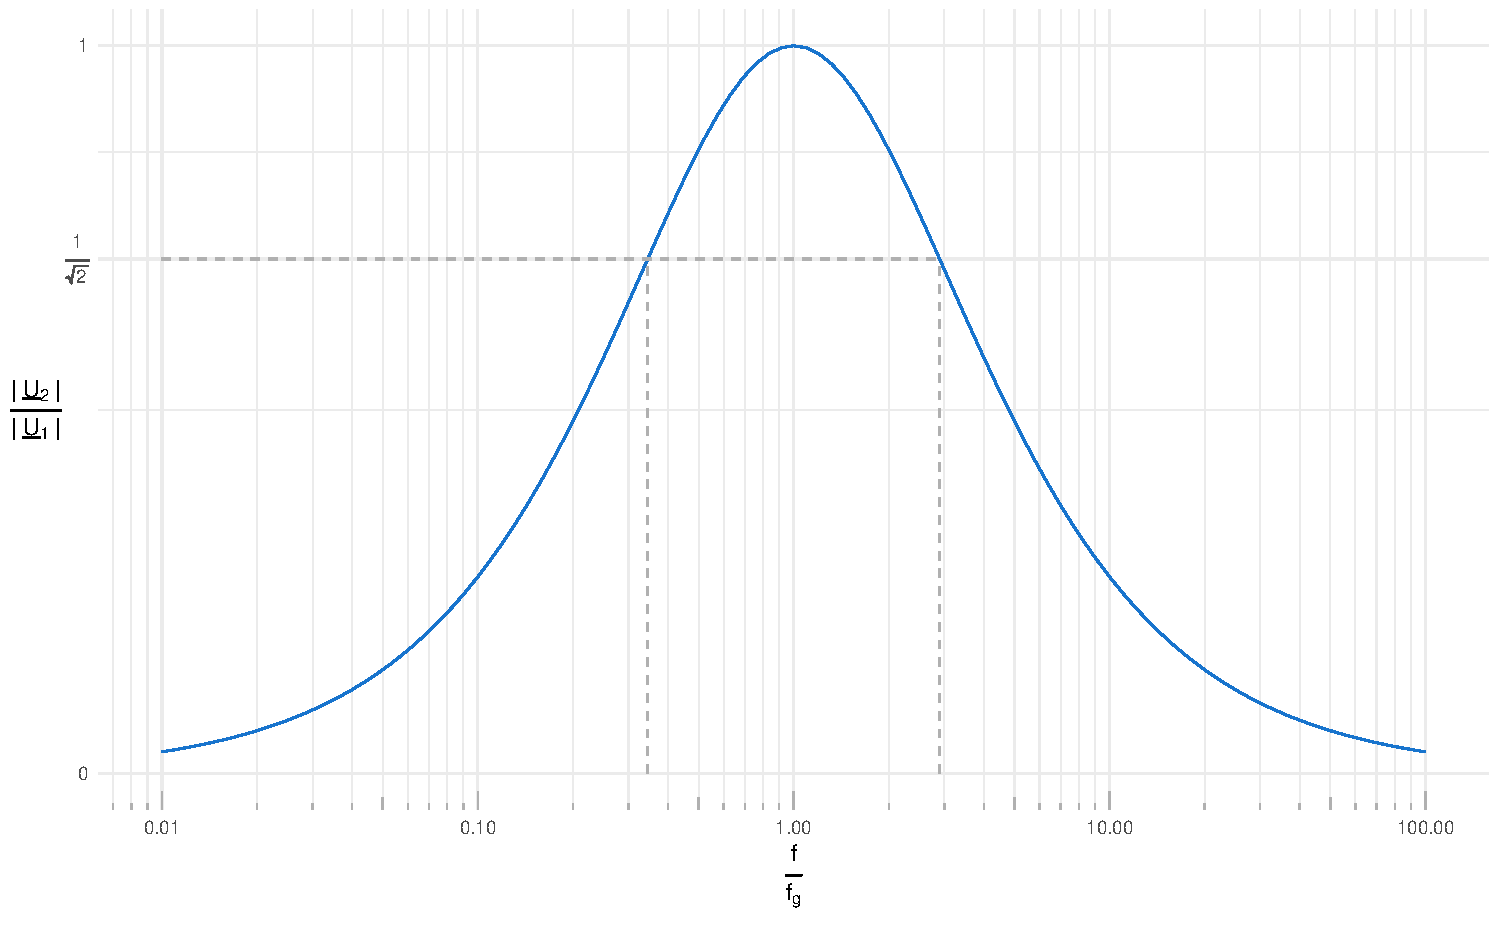
\includegraphics[scale=0.5]{./R/Band/BP/BP_clean.pdf}

  \vspace{0.021276873\paperheight}

  \subsubsection*{Bandsperre (BS)}

    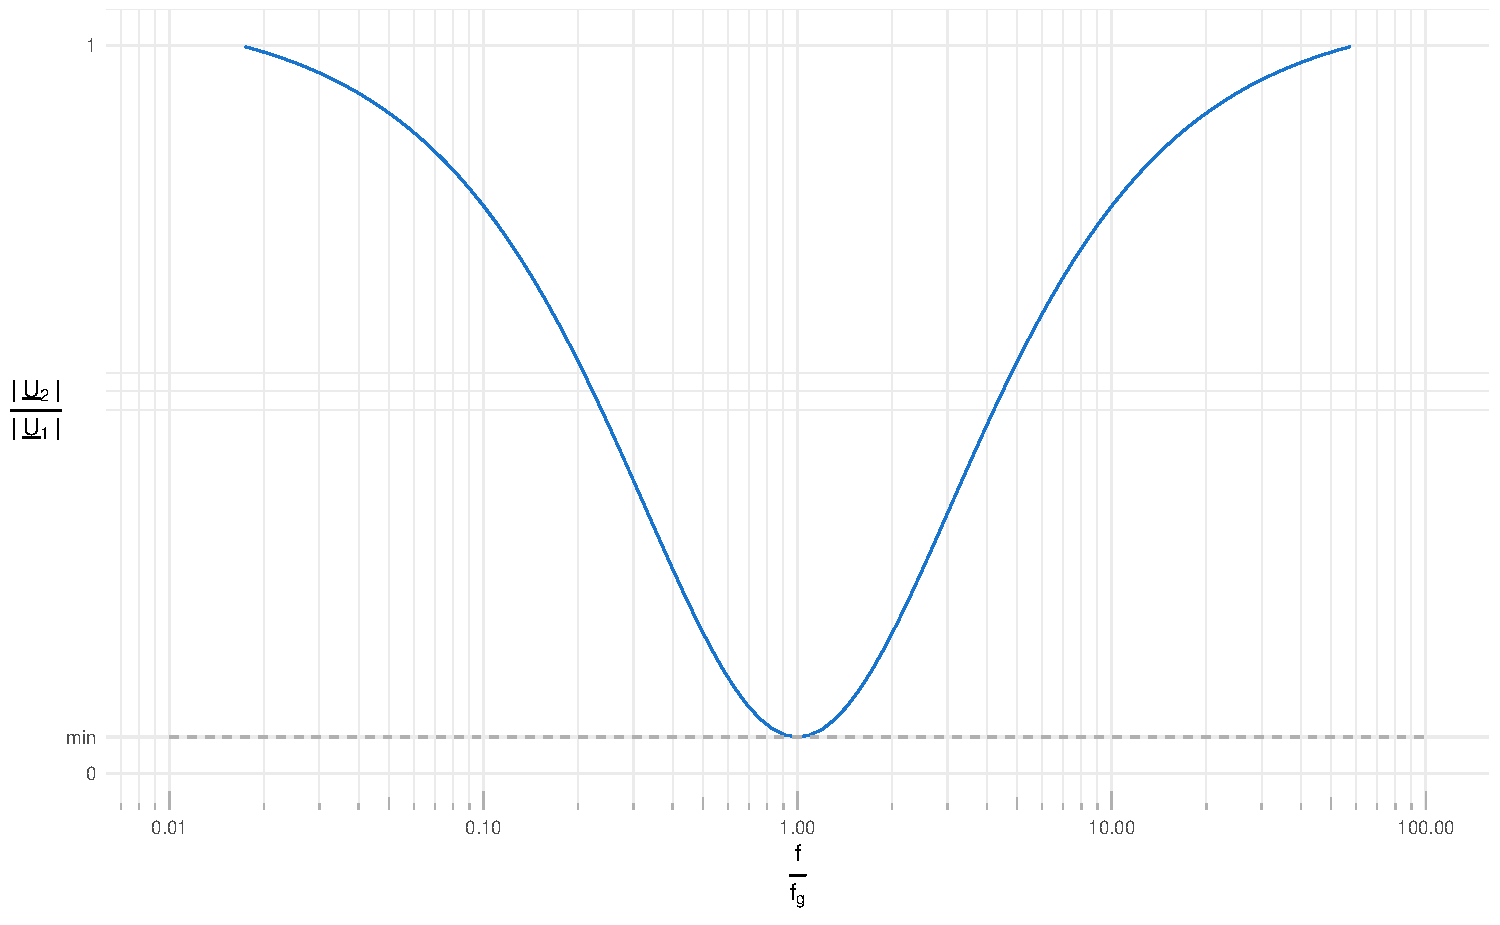
\includegraphics[scale=0.5]{./R/Band/BS/BS_clean.pdf}

  \end{center}

%1.6
\subsection{}
\subsubsection*{RC-Tiefpass}

  \begin{center}
    \begin{circuitikz}

      \draw (0,0) to[open,v^=$U_1$, o-o] (0,-3);
      \draw (.05,0) to[R, l=$R$] (4,0); % kinda hacked
      \draw (4,0) to[open] (6,0);
      \draw (4,0) -- (6,0);
      \draw (4,0) to[C, l=$C$, *-*] (4,-3);
      \draw (6,0) to[open,v^=$U_2$,o-o] (6,-3);
      \draw (5.95,-3) to[short] (0.05,-3);

    \end{circuitikz}
  \end{center}

  \begin{gather*}
    \frac{\underline{U}_2}{\underline{U}_1} = \frac{\frac{1}{j \omega C}}{R +\frac{1}{j \omega C}} = \frac{1}{j R \omega C + 1}\\
  \end{gather*}

\subsubsection*{RC-Hochpass}
\subsubsection*{RL-Tiefpass}
\subsubsection*{RL-Hochpass}

\subsection{}
\end{document}
